\documentclass[conference]{IEEEtran}

\usepackage{amsmath,amssymb}
\usepackage{amsfonts}
%\usepackage{amsthm} %proof environment
\usepackage{array} %better arrays and tabular
\usepackage{multirow} %single entry in multiple row elements in a tabular
\usepackage[para]{threeparttable} %add capability for additional notes to tables
\usepackage{booktabs} %nicer looking tabulars 
\usepackage{balance} %equalize the columns on the last page with \balance command
\usepackage[inline]{enumitem}
\usepackage{subfig}
\usepackage{graphicx}
\usepackage{cite}
\usepackage[vlined, ruled, linesnumbered, commentsnumbered]{algorithm2e}
 
\captionsetup[sub]{font=medium,labelfont={bf,sf}}

\interdisplaylinepenalty=2500 %Change amsmath definition back IEEEtran default

\newcommand{\bo}[1]{\boldsymbol{\mathrm{#1}}}
\newcommand{\norm}[1]{\lVert#1\rVert}
\newcommand{\Norm}[1]{\big \lVert#1\big\rVert}
\newcommand{\NORM}[1]{\left \lVert#1\right\rVert}
\newcommand{\abs}[1]{\lvert#1\rvert}
\newcommand{\Abs}[1]{\Big \lvert#1\Big \rvert}
\newcommand{\ABS}[1]{\bigg \lvert#1\bigg \rvert}
\newcommand{\re}{\mathrm{Re}}
\newcommand{\im}{\mathrm{Im}}
\newcommand{\tr}{\mathrm{trace}}
\newcommand{\diag}{\mathrm{diag}}
\newcommand{\dd}{\mathrm{d}}
\newcommand{\set}[1]{\mathcal{#1}}
\newcommand{\floor}[1]{\left\lfloor#1 \right\rfloor}
\newcommand{\iu}{\mathfrak{j}}

\newcommand{\thnoise}{\sigma^2_{\text{th}}}

\newcommand{\epower}{p_{m}}
\newcommand{\vpower}{\boldsymbol{p}}

\newcommand{\eintnoise}{\sigma^2_{\text{int}_{n}}}
\newcommand{\vintnoise}{\boldsymbol{\sigma}^2_{\text{int}}}

\newcommand{\esinr}{\gamma_{{nm}}}
\newcommand{\vsinr}{\boldsymbol{\gamma}}

\newcommand{\esinrexp}{\Gamma_{nm}}
\newcommand{\vsinrexp}{\boldsymbol{\Gamma}}

\newcommand{\esinrb}{\widehat{\Gamma}_{nm}}
\newcommand{\vsinrb}{\widehat{\boldsymbol{\Gamma}}}

\newcommand{\ereward}{r^t_a}
\newcommand{\vreward}{\boldsymbol{r}^t}

\newcommand{\brewardb}{B^{t_k}}
\newcommand{\vrewardb}{\boldsymbol{B}^t}

\newcommand{\epl}{L_{nm}}
\newcommand{\vpl}{\boldsymbol{L}}

\newcommand{\ercs}{\psi_{nm}}
\newcommand{\vrcs}{\boldsymbol{\psi}}

\newcommand{\fl}{c(t)}

\newcommand{\E}[1]{\mathbb{E}\left[ #1 \right]}

\newcommand{\easvtx}{\delta_{\text{tx}_m}}
\newcommand{\vasvtx}{\boldsymbol{\delta}_{\text{tx}}}
\newcommand{\easvrx}{\delta_{\text{rx}_n}}
\newcommand{\vasvrx}{\boldsymbol{\delta}_{\text{rx}}}
\newcommand{\vsp}{\boldsymbol{\rho}}
\newcommand{\esp}{\rho_{nm}}

\newcommand{\eindex}{X_{nm}}
\newcommand{\vindex}{\boldsymbol{X}}



\hyphenation{pa-ram-e-tr-iza-tion}

\title{Reinforcement Learning Based Transmitter-Receiver Selection for Distributed MIMO Radars}
\author{
	\IEEEauthorblockN{
        Petteri~Pulkkinen,
	    Tuomas~Aittom\"aki, and
        Visa~Koivunen%
	}
	\IEEEauthorblockA{
		Department of Signal Processing and Acoustics, \\
		Aalto University \\
		PO Box 15400, FI-00076 Aalto, Finland \\
	}
}


\begin{document}

\maketitle

\begin{abstract}

Active transmitter-receiver (TX-RX) subset selection facilitates efficient resource use and adaptation to varying target and propagation environments in distributed multiple-input multiple-output (MIMO) radar systems.
The problem has been addressed in the literature and objective functions related to radar tasks that depend on the signal-to-interference-plus-noise ratio (SINR) have been proposed. 
The SINR values observed at the receivers can be estimated assuming a particular propagation environment and target models. 
In this paper a novel machine learning approach is proposed in which no such assumptions are needed.
We formulate the TX-RX subset selection as a multi-armed bandit (MAB) problem and further extend it to the combinatorial MAB framework.
A variety of reinforcement learning algorithms developed for the MAB problem are employed to learn the optimal subset in real-time.
It is shown that such algorithms can be effectively used for the TX-RX subset selection problem even in non-stationary scenarios.

\end{abstract}

\begin{IEEEkeywords}
reinforcement learning, multi-armed bandits, subset selection, distributed MIMO radar
\end{IEEEkeywords}


%  -------------------------------------------------------------------------------
%   Introduction
%  -------------------------------------------------------------------------------
\section{Introduction}
\label{sec:intro}

A Distributed multiple-input and multiple-output (MIMO) radar is a system in which multiple transmitters and receivers are deployed in different locations \cite{Haimovich2008}.
The widely distributed antennas increase spatial diversity which can be utilized for improved target localization, parameter estimation and detecting low-observable targets.
In a MIMO radar, the used waveforms are designed jointly and the waveforms are typically orthogonal.
Therefore, each transmitter-receiver (TX-RX) pair forms an independent channel for illuminating and observing the targets.
Increasing the number of channels provides additional spatial diversity at the cost of larger amount of data to be processed and higher power consumption \cite{Godrich2011, Sun2014, Aittomaeki2018}.
In addition, active transmitters may expose their location which might be undesired in certain applications.
Strategies for TX-RX subset selection are studied to preserve the spatial diversity and reduce the costs at the same time.

The TX-RX subset selection problem, especially for target localization, has been previously addressed in the literature \cite{Godrich2011, Sun2014}.
In these studies, the signal-to-interference-plus-noise ratio (SINR) is assumed to be known or estimated.
It is possible to estimate the SINR based on assumed particular propagation environments and target models, but a real-world radar environment may deviate from the assumed model and consequently lead to performance degradation.

Another way to form the estimates is to probe the different channels for a sufficient number of times to learn their state. 
The probing needs to be efficient since the channels are continuously evolving and the probing will impact the radar performance because it requires performing extra tasks in addition to the main operation of the radar.  Therefore, it is necessary to decide when to exploit the TX-RX subset currently providing the best payoff or explore other subsets that may or may not provide even higher SINR levels. 
This is the exploration-exploitation trade-off.

This paper proposes a machine learning approach for the active TX-RX subset selection in the distributed MIMO radar context.
The problem is formulated as a multi-armed bandit (MAB) problem. 
The MAB framework provides policies for selecting actions to balance the exploration and exploitation trade-off while maximizing the employed reward function \cite{Lattimore2019}.
We use extensions from the combinatorial MAB framework to handle the exponentially growing action space and propose a generalized algorithm to solve the problem using any index-based MAB algorithm.



%  -------------------------------------------------------------------------------
%   Problem formulation
%  -------------------------------------------------------------------------------
\section{Problem formulation}

Assume a distributed MIMO radar system that consists of $N$ receivers and $M$ transmitters.
The radar system is constrained to use a subset of the transmitters and the receivers at the same time in order to save resources such as power and reduce the probability of being detected by an adversary.
Each TX-RX pair is considered as a channel and overall there are $K=NM$ channels.
The number of channels in a subset is $K_S = N_S M_S$, where both, the number of receivers $N_S$ and the number of transmitters $M_S$ in a subset are constrained with an equality constraint.
Selecting receiver $n \in \{1, 2, ..., N\}$ and transmitter $m \in \{1,2, ..., M\}$ is indicated with vectors $\vasvrx$ and $\vasvtx$ where
\begin{align}
    &\easvrx = 
    \left\{\begin{array}{l}
        1 \text{, when receiver $n$ is included in the set} \\
        0 \text{, otherwise}
    \end{array}\right.\\
    &\easvtx = 
    \left\{\begin{array}{l}
        1 \text{, when transmitter $m$ is included in the set} \\
        0 \text{, otherwise.}
    \end{array}\right.
\end{align}
Radar receivers are subject to both unintentional and intentional interference when observing target returns.
The quality of the received signal is typically characterized by signal-to-interference-plus-noise ratio (SINR).

In this paper, the measured signal power $\esp$ at receiver $n$ from transmitter $m$ via the target is modeled as a stochastic process that may be non-stationary. 
Non-stationary character of $\esp$ can stem from the target moving in the environment, and 
the movement causes variability to path losses and the radar cross-section (RCS).
Moreover, unintentional and intentional interference levels might change in time further contributing to the non-stationary behavior of the system.
It is assumed that sufficiently accurate estimates of the noise power $\thnoise$ and the interference power $\eintnoise$ at receiver $n$ are available.
Therefore, we can express the channel SINR on a linear scale as
\begin{equation}\label{eq:sinr}
     \esinrexp = \frac{\E{\esp}- (\thnoise + \eintnoise)}{\thnoise + \eintnoise },
\end{equation}
where the noise power and the interference power is subtracted from the received signal power and $\E{\esp} \geq \thnoise + \eintnoise$.
Note that the SINR is time dependent because random variable $\esp$ is non-stationary. 


Performance in target detection and target localization depend on the SINR level \cite{aittomaki1, aittomaki2, antenna_subset_selection, selection_and_placement}.
Therefore, a reward function for reinforcement learning is proposed that depends on the vector $\vsinrexp$ that consists of all the SINR values $\esinrexp$.
The following reward function is used for the employed MAB learning
\begin{equation}\label{eq:reward_func}
    r(\vasvrx, \vasvtx | \vsinrexp) = \frac{1}{N_S M_S}\sum_{n=1}^N \sum_{m=1}^M  \easvrx \easvtx \esinrexp,
\end{equation}
which is a mean of SINR values for the selected channels on a linear scale.
Furthermore, the reward maximization problem can be formulated as
\begin{equation}\label{eq:obj_func}
    \begin{array}{ll}
                &   \max_{\vasvrx, \vasvtx} r(\vasvrx, \vasvtx | \vsinrexp) \\[7pt]
    \text{s.t.} &   
                \left\{\begin{array}{l}
                    \sum_{n=1}^N \easvrx = N_S \\
                    \sum_{m=1}^M \easvtx = M_S.
                \end{array}\right.
    \end{array}
\end{equation}
It is possible to find an optimal solution for the equation (\ref{eq:obj_func}) if $\vsinrexp$ is known.
However, $\vsinrexp$ is not known since we can only obtain the measurements $\esp$. 
Furthermore, it might not be possible to probe all the channels at the same time.
Therefore, $\vsinrexp$ needs to be estimated from the received signal. 
By probing the different channels, an estimate $\vsinrb$ of the channel SINR values can be formed.
An approximate solution for the objective (\ref{eq:obj_func}) is found when the estimate $\vsinrb$ is used to condition the reward function (\ref{eq:reward_func}).
Different subsets must be explored sufficiently large number of times to reinforce the estimate $\vsinrb$ to identify the subset of TX-RX pairs yielding the highest SINR values.

%  -------------------------------------------------------------------------------
%   Multi-armed bandits
%  -------------------------------------------------------------------------------
\section{Multi-armed bandits}
\label{sec:mab}

The MAB problem is a sequential decision-making problem in which an agent needs to decide on an action from several competing actions \cite{rl_intro}.
The word arm originates from a slot machine that has a pull lever, and the pull lever is called an arm.
Pulling an arm of a slot machine gives a reward based on a certain probability distribution.
In the MAB problem, the agent needs to sequentially decide from many arms which arm to pull to maximize the cumulative reward.
The strategy of how the agent chooses the arms is called a policy.

Usually, the performance for a policy is measured with regret.
The regret quantifies the cost of learning by measuring how much reward agent has missed from the cumulative reward.
In this paper, the performance for policy $\pi$ is measured with normalized regret
\begin{equation}\label{eq:reg}
    R_\pi(T) = \sum_{t=1}^T \left( 1 - \frac{\mu^\pi_t}{\mu^*_t} \right),
\end{equation}
where $T$ is the time horizon, $\mu^\pi_t$ is the expected reward for the policy $\pi$ at time instant $t$ and $\mu_t^*$ is the expected reward for the optimal arm at time instant $t$.
Moreover, the normalized regret describes how large proportion of the optimal reward is missed at each iteration, which is useful when the rewards are non-stationary.
Sublinear regret as a function of $T$ indicates that the agent has made choices in previous time instances that improve the future choices.

To maximize the cumulative reward, the agent needs to find the arm which gives the highest expected reward.
This means that the agent needs to decide when to explore different arms to possibly identify those with higher expected rewards 
and when to keep pulling the arm with currently known highest expected reward.
An estimate for the expected reward is updated each time when the agent has pulled an arm.
The update equation for each arm can be written as
\begin{equation}\label{eq:update1}
    q_{t+1}(a) = q_{t}(a) + \alpha \left(r_t + q_{t}(a)\right),
\end{equation}
where $r_t$ is the received reward from selecting the arm $a$, $\alpha$ is a step size and $q_{t}(a)$ is called action-value \cite{rl_intro}.
For stationary rewards, $\alpha$ can be set to $t^{-1}$, so that (\ref{eq:update1}) calculates the empirical mean. 
For non-stationary rewards, the parameter $\alpha$ needs to be constant so that old rewards have a lower weight than more recent ones \cite{rl_intro}.

In practice, a policy is realized as an algorithm.
We briefly review five different MAB algorithms which are used in the simulations.
The selected algorithms are widely used to solve MAB problems.
These algorithms are
\begin{enumerate}
    \item $\epsilon$-greedy \cite{rl_intro},
    \item Upper Confidence Bound (UCB1) \cite{rl_intro, DSWUCB},
    \item Kullback Leibler Upper Confidence Bound (KL-UCB) \cite{KL_UCB},
    \item Thompson sampling \cite{Thompson, DThompson} and
    \item Recency-Based Exploration (RBE) \cite{RBE,DRBE}.
\end{enumerate}
An analysis for stationary and non-stationary reward distributions can be found in the references.
Also, other algorithms and more extensive discussion on the multi-armed bandits can be found in \cite{lattimorebandit, rl_intro, mab_survey, intro_to_mab}.

In the $\epsilon$-greedy algorithm the probability of choosing a random arm is $0 < \epsilon \ll 1$ and this probability remains constant in time.
When not selecting an arm randomly, the algorithm chooses the arm which has the highest action-value.
The UCB1 and KL-UCB are policies which are based on deriving an upper confidence bound for the expected rewards and the arm with highest bound is selected.
Thompson sampling is Bayesian algorithm where the posterior probability distributions for the expected rewards are formed from the collected rewards.
Then the posterior distributions are sampled at each time instant and the arm with the highest sample is selected.
Finally, the RBE is based on defining an exploration term to support choosing arms which have not been explored recently.
In addition, the term is constructed in a way that the agent prefers arms which have the highest action-values.

Most of the MAB algorithms such as UCB1, KL-UCB, Thompson sampling and RBE are index-based polices that calculate a measure, called an index, for each arm.
The index captures the uncertainty on the action-value $q_t(a)$ and emphasizes exploration for those arms that might have desirable expected rewards.
Typically, the index is constructed in a way that the arm with highest index is selected.

Another way to solve a MAB problem is to divide the exploration and the exploitation into two distinct phases.
This division can be fully deterministic or random. 
Deterministic algorithms divide the exploration and the exploitation phases into blocks of specific lengths \cite{lattimorebandit}.
Random algorithms, such as $\epsilon$-greedy, explore different arms with some probability and otherwise they exploit the arm with currently highest action-value. 

%  -------------------------------------------------------------------------------
%   Formulation as a multi-armed bandit problem
%  -------------------------------------------------------------------------------
\section{Multi-armed bandit problem formulation}
\label{sec:fmab}

Classical multi-armed bandits have a finite set of arms and a single arm is selected at each time instant.
Each subset of TX-RX pairs could be one arm associated with the reward given by the objective function.
However, a number of the arms would be $\binom{N}{N_S}\binom{M}{M_S}$ which grows exponentially. This could make the problem unsolvable with the MAB approach because there is no time to explore all the arms in a given time horizon.
The amount of time which is available for learning the different channels depends on the dynamic nature of targets and the propagation scenario.
For example, if a target appears or disappears or does abrupt maneuvers, then rapid changes in the reward distributions will happen. 
On the other hand, smooth changes take place when a target moves on a smooth trajectory and changes its orientation gradually.

The problem with exponentially increasing number of arms can be avoided by reformulating the MAB model so that each arm represents SINR for each channel and the agent can choose multiple arms at each time instant.
The arms are chosen to maximize the reward function and satisfy the constraints.
When this formulation is used, the action-values introduced in section~\ref{sec:mab} are the channel SINR estimates $\vsinrb$.
The total number of arms is reduced to $NM$ and the agent can choose $N_S M_S$ arms at each iteration.
The formulation is known as the combinatorial multi-armed bandits, in which the subset of arms is called a super arm \cite{comb_mab}.
The reformulation is possible because the reward function ($\ref{eq:obj_func}$) is an increasing function of the radar channel SINR values and each arm is independent since waveforms from different transmitters do not interfere with each other if orthogonal waveforms are used.

Usually in the combinatorial MAB problem, the agent does not know the mapping from the arm rewards to the super arm rewards.
However, here the reward function $\eqref{eq:reward_func}$ is known which enables us to use MAB algorithms from the classical MAB problem.
Similar approach is used for MIMO antenna subset selection in mobile communications, where each arm represents power-normalized throughput for each antenna and UCB1-algorithm paired with an exhaustive search were used to solve the subset selection problem \cite{MAB_subset_selection}.
The reward distributions were assumed stationary in \cite{MAB_subset_selection}.  

In this paper we generalize the approach in \cite{MAB_subset_selection} to any index-based algorithm and non-stationary reward distributions. 
The proposed algorithm for solving the combinatorial MAB problem with known mapping from the arm rewards to the super arm rewards is shown in Algorithm~\ref{alg:gcmab}.
The algorithm allows for using any optimization method to find the super arm, and any index-based MAB algorithm to find the indexes.
The indexes calculated by a MAB algorithm will ensure that the exploration and exploitation trade-off is balanced well.

The principles of the Algorithm~\ref{alg:gcmab} can be also used for the random policies by using the SINR estimates $\vsinrb$ instead of the indexes.
In addition, random policies explore different subsets by selecting them randomly.
However, the exploration is not as efficient as with index-based policies, because the fact that the super arm rewards are a function of the arm rewards is not utilized.

\begin{algorithm}[h]
\SetAlgoLined
\While{not end of the time horizon}{
calculate indexes for all arms\;
find the super arm using the indexes\;
pull the super arm\;
\If {non-stationary rewards}{
discount rewards for all arms\;
discount exploration parameters for all arms\;
}
observe the arm rewards\;
update the arm rewards\; 
update the exploration parameters\;
}
\caption{Proposed generalized algorithm}
\label{alg:gcmab}
\end{algorithm}

%  -------------------------------------------------------------------------------
%   Simulation setup
%  -------------------------------------------------------------------------------
\section{Simulation setup}
\label{sec:sim}


\subsection{System Configuration}
\label{seq:sys_conf}
The simulated MIMO radar system consists of $N=6$ receivers and $M=4$ transmitters.
A subset with $N_S=3$ receivers and $M_S=2$ transmitters is selected, so that six out of 24 possible channels are used at any time instance.
It is possible to use exhaustive search to find the super arm because there are only 120 different subsets.
The simulation environment is visualized in Fig.\ref{fig:env}.

\subsection{Scattering Model}
\label{seq:sc_model}

The target illumination angle and the scattering angle are usually different for each TX-RX pair in distributed MIMO radars.
Therefore, the RCS model depends on the angles to the receiver and the transmitter.
The dependency on the angles for receiver $n$ and transmitter $m$ is denoted by $\ercs$ which is a product between two scattering coefficients that are taken from the monostatic target RCS model at the illumination angle and the scattering angle.
The simplistic monostatic RCS model used in simulations is expressed by a simple sum of cosine functions $0.064 \cdot \abs{2.5\cos(\theta) + 7\cos(2\theta) + 3\cos(3\theta) + 3\cos(4\theta)}$, where $\theta$ is the backscatter angle.

The target RCS fluctuation is modeled based on the Swerling I model.
Hence, the power loss of the target fluctuation $c$ is modeled by the exponential distribution with the scale parameter equal to one, and $c$ remains constant between two subsequent time instances.

\subsection{Propagation Environment Model}
\label{seq:env_model}

The environment model includes path losses, thermal noise, and external interference.
The path loss $\epl = d_\text{tx}^{-2} d_\text{rx}^{-2}$ is a product between
reciprocal of targets' squared distance to the transmitter and the receiver.
The thermal noise power $\thnoise=0.001$ is constant in time and the same for all the channels.
Also, the interference power $\vintnoise=[0.1, 0.9, 0.3, 0.1, 0.2, 0.4]^T$ is constant in time and $\eintnoise$ is the interference power at receiver~$n$.

\begin{figure}[!tb]
    \centering
    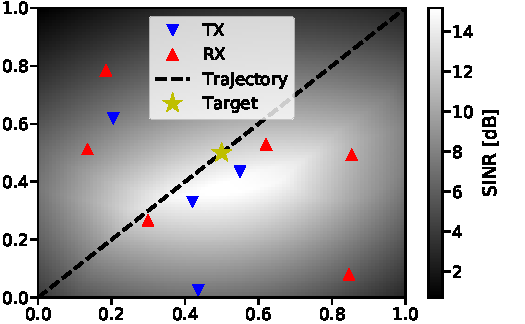
\includegraphics{figures/env.pdf}
    \caption{Simulation setup.
    The target position is shown for the stationary case and the trajectory for the non-stationary case. 
    The heat map indicates the mean channel SINR at every position when the target scattering coefficient is excluded and all the channels are active.}
    \label{fig:env}
\end{figure}

\subsection{Rewards}

The agent aims to find the super arm which has the highest reward based on the equation \eqref{eq:reward_func}. 
To create the arm rewards, we define an instantaneous SINR measure $\esinr$ that satisfies $\E{\esinr} = \esinrexp$ where $\esinrexp$ is the channel SINR. 
The value $\esinr$ is calculated using the equation \eqref{eq:sinr} where the expectation is replaced with the power measurement $\esp$. 
To simplify the simulations, 
the target scattering coefficient remains constant through a single measurement period and the stochasticity of the noise and the interference powers in the measurements are approximated to be negligible. 
Therefore, the rewards for each arm are simulated by
\begin{equation}
    \esinr  = \esinrexp c \sim \text{Exp}\left(\frac{1}{\esinrexp}\right),
\end{equation}
which is the exponential distribution with mean of $\esinrexp$.
The channel SINR $\esinrexp$ on a linear scale for receiver $n$ and transmitter $m$ is calculated from the models defined in sections \ref{seq:sys_conf} \ref{seq:sc_model} and \ref{seq:env_model} as follows
\begin{equation}
    \esinrexp = \frac{\epl \ercs \epower}{\thnoise + \eintnoise},
\end{equation}
where the transmit power $\epower=1$ is constant in time and equal for each transmitter.



\begin{figure}[!tb]\centering
    \subfloat[Stationary case.]
    {
        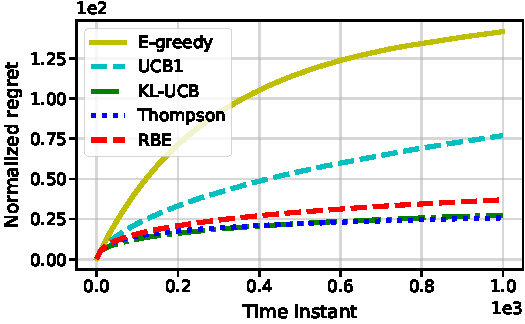
\includegraphics[width=.9\columnwidth]{figures/stationary/cmab/regret.pdf}
        \label{fig:stationary_regret}
    }
    \hfill
    \subfloat[Non-stationary case.]
    {
        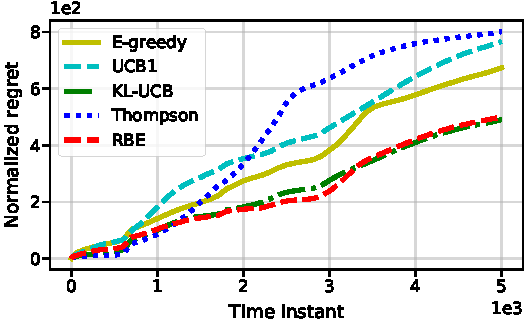
\includegraphics[width=.9\columnwidth]{figures/non_stationary/regret.pdf}
        \label{fig:non_stationary_regret}
    }
    \caption{The normalized regret at each time instant. 
            RBE and KL-UCB perfom well in the both cases.}
    \label{fig:regret}
\end{figure}

\begin{figure}[!tb]\centering
    \subfloat[Stationary case.]
    {
        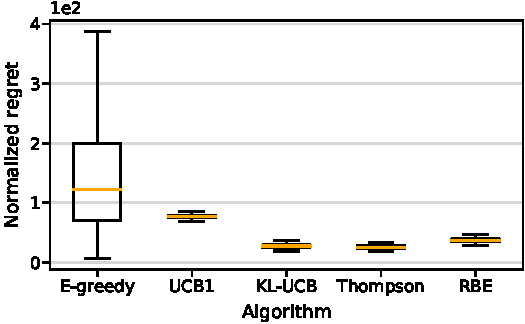
\includegraphics[width=.9\columnwidth]{figures/stationary/cmab/regret_box.pdf}
        \label{fig:stationary_ci}
    }
    \hfill
    \subfloat[Non-stationary case.]
    {
        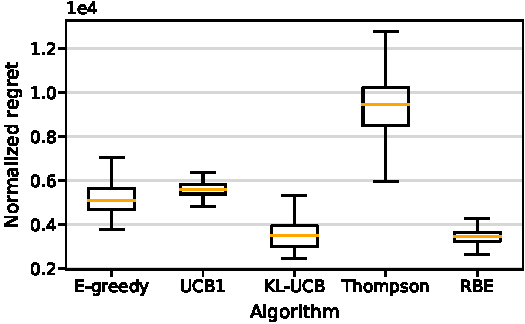
\includegraphics[width=.9\columnwidth]{figures/non_stationary/regret_box.pdf}
        \label{fig:non_stationary_ci}
    }
    \caption{The normalized regret for the whole time horizon compared between different simulation runs.
            RBE and KL-UCB obtain excellent results in both stationary and non-stationary scenarios.}
    \label{fig:ci}
\end{figure}

\begin{figure}[!tb]
    \subfloat[Stationary case.]
    {
        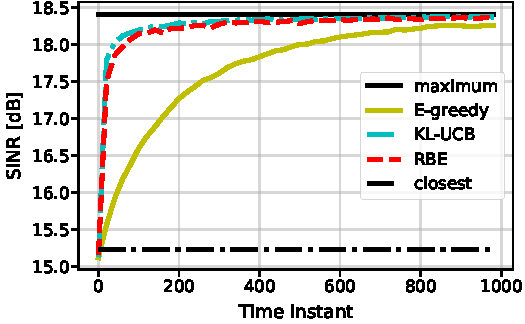
\includegraphics[width=.9\columnwidth]{figures/stationary/cmab/sinr.pdf}
        \label{fig:stationary_sinr}
    }
    \hfill
    \subfloat[Non-stationary case.]
    {
        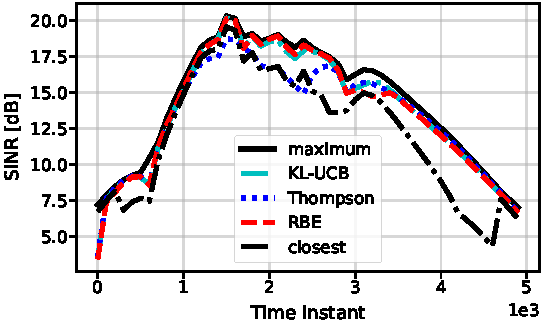
\includegraphics[width=.9\columnwidth]{figures/non_stationary/sinr.pdf}
        \label{fig:non_stationary_sinr}
    }
    \caption{Reward at each time instant.
    The reward is a mean of the channel SINRs in a linear scale for the selected subset.
    The MAB algorithms are compared to a simple exploration-free method in which the subset of the receivers and the transmitters closest to the target is selected.
    In average, most of the MAB algorithms achieve a reward close to the maximum reward.}
    \label{fig:sinr}
\end{figure}


%  -------------------------------------------------------------------------------
%   Simulation results
%  -------------------------------------------------------------------------------
\section{Simulation results}

Two different scenarios are studied in the simulation examples. 
In the stationary scenario, there is a target that remains stationary at position $(0.5, 0.5)$.
In the non-stationary scenario, a target moves from $(0, 0)$ to $(1, 1)$ on a linear trajectory with a constant velocity.
All other parameters for the environment remain the same in both scenarios.
The five algorithms that were briefly reviewed in section~\ref{sec:mab} are used in the simulations.
The performances of the different MAB algorithms were evaluated using Monte Carlo simulations with $1000$ iterations.

A simple method that selects the closest subset at each time instant is proposed to compare the MAB algorithms to a more conventional exploration-free method. 
The comparison is performed by comparing expectation of the achieved rewards through the simulation period. 

The achieved rewards for two well-functioning MAB algorithms, 
the worst MAB algorithm and the exploration-free method are shown in Fig.~\ref{fig:sinr}. 
The MAB algorithms are compared between each other in terms of regret. 
The regret through the simulation period is shown in Fig~\ref{fig:regret}. 
Also, box plots of the regrets are shown in Fig~\ref{fig:ci}.
The overall results show that the MAB algorithms improve the performance through the time horizon and outperform the exploration-free method in stationary and non-stationary cases.
Moreover, the RBE algorithm stands out with excellent reliability and regret performance in both cases.

\subsection{Stationary target}

In the stationary case, the discount factor can be set to $\alpha=t^{-1}$.
The value of $\epsilon$ for $\epsilon$-greedy exploration is set to 0.1, which means that it explores random subsets 10\% of the time.
Lower $\epsilon$ can sometimes result in lower regret, but the variance of the regret may increase.
The value 0.1 was found empirically in this simulation.
The other algorithms do not have any tunable parameters.
The time horizon is set to 1000 which is sufficiently long for finding the optimal TX-RX configuration.

The stationary target implies that the expected rewards of the arms do not change in time.
Therefore, it is possible to achieve a logarithmic regret \cite{lattimorebandit}.
From Fig.\ref{fig:stationary_regret} it can be observed that all algorithms other than $\epsilon$-greedy can achieve the sublinear regret.
Algorithms like Thompson sampling and KL-UCB which require knowledge about the reward distribution have excellent performance in these simulations.
The $\epsilon$-greedy algorithm has the highest regret and it is visible from Fig.\ref{fig:stationary_ci} that such random policies have a high variance.
Algorithms with higher variance make the learning less reliable even though they can some times find the optimal action faster than more reliable algorithms.

Fig.$\ref{fig:stationary_sinr}$ visualizes the achievable reward at each time instant.
The main difference between the MAB algorithms is the time taken to find the optimal super arm.
The gap between the maximum achievable reward and achieved expected reward will decrease as a function of time for algorithms that achieve sublinear regret.
Therefore, $\epsilon$-greedy with constant exploration probability will eventually have a constant gap between maximum reward and achievable expected reward.
It can be observed that the MAB algorithms perform much better than the exploration-free method.

\subsection{Non-stationary target}


For the non-stationary case, the path-losses $\vpl$ and the angle-dependent scattering coefficients $\vrcs$ change in time.
In other words, the instantaneous SINR values $\vsinr$ are non-stationary and the channel SINR values $\vsinrexp$ are time-dependent.
The algorithms adapt to the non-stationary conditions by using the discounted action-value and discounted exploration parameters.
The discount factor is set to $\alpha = 0.998$.
Also, each element of $\vsinrb$ is divided by the maximum value before calculating the index.
This ensures that enough exploration is done at each time instant even if the scale of the rewards changes over time.
The value of $\epsilon$ for $\epsilon$-greedy algorithm is kept at 0.1.
The asymptotic optimality can not be achieved since the exploration term will never vanish completely.
However, the considered algorithms have differences in their exploration efficiencies, as can be observed from the different regrets in Fig.\ref{fig:non_stationary_regret}.

In Fig.~\ref{fig:non_stationary_regret} it can be seen that KL-UCB and RBE achieve the lowest regret in the non-stationary case.
Thompson sampling does not adapt as well for the non-stationary case even if it performed quite well in the stationary case.
The $\epsilon$-greedy algorithm has lower regret than Thompson sampling but it still performs worse than the other algorithms. 
The Fig.\ref{fig:non_stationary_ci} demonstrates that RBE algorithm has a very small regret with low variance.
Also, the median performance is better than with any other of the used algorithms.
Hence it is very promising algorithm for the radar problem at hand. 
The other algorithms which performed well in stationary reward scenario have poorer performance in non-stationary reward case.
The changes in reward distributions will force the agent to switch the arm if the action-value for the arm under exploitation becomes lower than the other action-values.
Therefore, in case of non-stationary target, the $\epsilon$-greedy algorithm achieves a smaller variance on regret than with stationary targets.

The achieved rewards are compared in Fig.\ref{fig:non_stationary_sinr}.
All MAB algorithms perform on average better than the exploration-free method through the whole simulation period.
Also, it is visible that the MAB algorithms can reach a SINR value close to the maximum reward at most of the time instances. 
Moreover, the performance gap between MAB algorithms is not as significant as in the stationary scenario.


%  -------------------------------------------------------------------------------
%   Conclusions
%  -------------------------------------------------------------------------------
\section{Conclusions}
\label{sec:concl}
The transmitter-receiver subset selection problem, in which the channel SINR values are unknown, was considered for the distributed MIMO radars.
Since only a subset of the channels can be selected at the same time, it was shown that such problems have to deal with the exploration and exploitation trade-off to identify the optimal subset without degrading the radar performance.
The problem was formulated as the combinatorial multi-arm bandit problem and reinforcement learning algorithm was proposed to solve the problem.
It was shown that reinforcement learning can be effectively used to continuously improve the subset selections and outperform the proposed exploration-free method.

\bibliographystyle{IEEEtran}
\bibliography{references}

\balance

\end{document}



